\documentclass[12pt,a4paper,oneside]{report}

% ======================================================
% 1. CẤU HÌNH GÓI LỆNH (PACKAGES)
% ======================================================
\usepackage[utf8]{inputenc}
\usepackage[vietnamese]{babel}
\usepackage{amsmath}
\usepackage{amsfonts}
\usepackage{amssymb}
\usepackage{graphicx}
\usepackage{indentfirst}
\usepackage{geometry}
\geometry{a4paper, left=3cm, right=2cm, top=2.5cm, bottom=2.5cm}
\usepackage{titlesec}
\usepackage{listings}
\usepackage{xcolor}
\usepackage{hyperref}
\usepackage{setspace}
\usepackage[most]{tcolorbox}
\usepackage{tikz}
\usetikzlibrary{calc}
\usepackage{fancyhdr}
\usepackage{float} 

% --- Dãn dòng chuẩn học thuật (1.3 tương đương 1.5 lines Word) ---
\linespread{1.3}

% --- CẤU HÌNH ĐẦU TRANG VÀ CHÂN TRANG ---
\pagestyle{fancy}
\fancyhf{} 
\fancyhead[L]{\small TRƯỜNG ĐẠI HỌC BÁCH KHOA} 
\fancyhead[R]{\small ĐỒ ÁN LẬP TRÌNH TÍNH TOÁN}
\fancyfoot[L]{\textit{Trần Văn Trường Vũ -- Trần Ngọc Bảo Quyên}} 
\fancyfoot[R]{\textbf{\thepage}} 
\renewcommand{\headrulewidth}{0.6pt} 
\renewcommand{\footrulewidth}{0.6pt} 

\fancypagestyle{plain}{
    \fancyhf{}
    \fancyhead[L]{\small TRƯỜNG ĐẠI HỌC BÁCH KHOA} 
    \fancyhead[R]{\small ĐỒ ÁN LẬP TRÌNH TÍNH TOÁN}
    \fancyfoot[L]{\textit{Trần Văn Trường Vũ -- Trần Ngọc Bảo Quyên}}
    \fancyfoot[R]{\textbf{\thepage}}
    \renewcommand{\headrulewidth}{0.6pt}
    \renewcommand{\footrulewidth}{0.6pt}
}

% --- CẤU HÌNH TIÊU ĐỀ CHƯƠNG MỤC THEO MẪU KHOA CNTT ---
\titleformat{\chapter}[hang]{\bfseries\Large\color{black}}{\thechapter.}{0.5em}{\MakeUppercase}
\titlespacing*{\chapter}{0pt}{-10pt}{15pt}
\titleformat{\section}[hang]{\bfseries\large}{\thesection.}{0.5em}{}
\titleformat{\subsection}[hang]{\bfseries\normalsize}{\thesubsection.}{0.5em}{}
\titleformat{\subsubsection}[hang]{\bfseries\normalsize\itshape}{\thesubsubsection.}{0.5em}{}

% --- CẤU HÌNH MÀU SẮC MÃ NGUỒN (CODE) ---
\definecolor{codegreen}{rgb}{0,0.6,0}
\definecolor{codegray}{rgb}{0.5,0.5,0.5}
\definecolor{codepurple}{rgb}{0.58,0,0.82}
\definecolor{backcolour}{rgb}{0.98,0.98,0.95}

\lstdefinestyle{UserCStyle}{
    backgroundcolor=\color{backcolour},   
    commentstyle=\color{codegreen}\itshape,
    keywordstyle=\color{blue}\bfseries,
    numberstyle=\tiny\color{codegray},
    stringstyle=\color{codepurple},
    basicstyle=\footnotesize\ttfamily,
    breakatwhitespace=false,         
    breaklines=true,                 
    captionpos=b,       
    keepspaces=true,                 
    numbers=left,                    
    numbersep=5pt,                  
    showspaces=false,               
    showstringspaces=false,
    showtabs=false,                  
    tabsize=4,
    language=C++
}

\begin{document}

% ==================== TRANG BÌA CÓ KHUNG VIỀN ĐÔI ====================
\begin{titlepage}
\begin{tikzpicture}[remember picture, overlay]
    % Vẽ đường viền dày phía ngoài
    \draw[line width = 1.5pt, draw=blue!40!black] 
        ($(current page.north west) + (2.5cm,-2.0cm)$) 
        rectangle 
        ($(current page.south east) + (-1.5cm,2.0cm)$);
    % Vẽ đường viền mảnh chạy song song phía trong
    \draw[line width = 0.5pt, draw=blue!40!black] 
        ($(current page.north west) + (2.65cm,-2.15cm)$) 
        rectangle 
        ($(current page.south east) + (-1.65cm,2.15cm)$);
\end{tikzpicture}

\begin{center}
    {\large \textbf{TRƯỜNG ĐẠI HỌC BÁCH KHOA}} \\
    {\large \textbf{KHOA CÔNG NGHỆ THÔNG TIN}} \\
\textbf{---------- o0o ----------} \\
\vspace{1.5cm}
    \begin{figure}[H]
        \centering
        % NẾU CÓ ẢNH LOGO TRƯỜNG THÌ BỎ DẤU % Ở DÒNG DƯỚI ĐỂ HIỂN THỊ
        
\includegraphics[width=0.25\textwidth]{Picture/itf.jpg} 
        % \fbox{\begin{minipage}{4cm}\centering\vspace{1.5cm}\textbf{LOGO KHOA}\vspace{1.5cm}\end{minipage}}
    \end{figure}
    \vspace{1.5cm}
    {\Large \textbf{ĐỒ ÁN LẬP TRÌNH TÍNH TOÁN}} \\
    \vspace{1.5cm}
    {\Large \bfseries \color{blue!60!black} XÂY DỰNG CHƯƠNG TRÌNH TÌM ĐƯỜNG ĐI NGẮN NHẤT TRÊN ĐỒ THỊ CÓ HƯỚNG CÓ TRỌNG SỐ} \\
    
    \vspace{3cm}
    
    \begin{flushleft}
    \hspace{1.5cm}
    \begin{tabular}{lll}
        \textbf{Người hướng dẫn:} & \textbf{ThS. TRẦN HỒ THỦY TIÊN} & \\
        \textbf{Sinh viên thực hiện:} & Trần Văn Trường Vũ & LỚP: 25Nh.11A \\
        & Trần Ngọc Bảo Quyên & LỚP: 25Nh.11A \\
    \end{tabular}
    \end{flushleft}
    
    \vfill
    {\large \textbf{Đà Nẵng, 06/2026}}
\end{center}
\end{titlepage}

% ==================== MỤC LỤC & DANH MỤC ====================
\newpage
\pagenumbering{roman}

\tableofcontents
\addcontentsline{toc}{chapter}{\contentsname}

\newpage
\renewcommand{\listfigurename}{DANH MỤC HÌNH VẼ}
\listoffigures
\addcontentsline{toc}{chapter}{\listfigurename}

% ==================== PHẦN MỞ ĐẦU ====================
\newpage
\pagenumbering{arabic}
\chapter*{MỞ ĐẦU}
\addcontentsline{toc}{chapter}{MỞ ĐẦU}

\section*{1. Mục đích thực hiện đề tài}
Trong kỷ nguyên công nghệ số và sự phát triển mạnh mẽ của các hệ thống mạng lưới, bài toán tối ưu hóa đường đi trên đồ thị đóng vai trò cốt lõi trong nhiều lĩnh vực thực tiễn. Phần mềm hỗ trợ trực quan hóa giúp công việc thiết kế, phân tích và học tập trở nên tối ưu và thân thiện hơn. Đề tài này được thực hiện nhằm mục đích giúp nhóm sinh viên rèn luyện tư duy thiết kế giải thuật hợp lý, hiện thực hóa các kiến thức cốt lõi đã học trong học phần Toán rời rạc, Kỹ thuật lập trình và Cấu trúc dữ liệu để giải quyết một bài toán thực tiễn phức tạp. 

\section*{2. Mục tiêu đề tài}
Mục tiêu trung tâm của đồ án là phân tích chuyên sâu, thiết kế và thực thi ứng dụng tìm đường đi ngắn nhất giữa hai điểm bất kỳ trên đồ thị có hướng có trọng số. Các mục tiêu cụ thể bao gồm:
\begin{itemize}
    \item \textbf{Xử lý dữ liệu linh hoạt:} Thiết lập module tự động đọc và phân tích cấu trúc ma trận kề từ tệp tin văn bản định dạng tĩnh.
    \item \textbf{Cài đặt thuật toán chính xác:} Áp dụng và tối ưu hóa giải thuật Dijkstra để tính toán nhãn đường đi tối ưu, đồng thời lưu vết phục vụ truy xuất lộ trình logic.
    \item \textbf{Mô phỏng đồ họa trực quan:} Tích hợp thư viện đồ họa Raylib để thiết kế không gian tương tác động, biểu diễn quá trình loang duyệt đỉnh một cách sinh động nhất.
\end{itemize}

\section*{3. Phạm vi và đối tượng nghiên cứu}
\begin{itemize}
    \item \textbf{Đối tượng nghiên cứu:} Cơ sở toán học của đồ thị có hướng, thuật toán tối ưu hóa nhãn Dijkstra, cấu trúc dữ liệu ma trận kề, phương trình hình học tọa độ vector và nguyên lý máy trạng thái (State Machine).
    \item \textbf{Phạm vi nghiên cứu:} Vận dụng tổng hợp ngôn ngữ lập trình C/C++ thuần túy kết hợp thư viện Raylib. Giới hạn trên mô hình đồ thị có trọng số cạnh không âm (điều kiện hội tụ của thuật toán Dijkstra).
\end{itemize}

\section*{4. Phương pháp nghiên cứu}
Đồ án vận dụng phương pháp nghiên cứu lý thuyết kết hợp thực nghiệm. Nhóm đã tiến hành khảo sát các giáo trình Toán rời rạc chuyên ngành, nghiên cứu tài liệu lập trình đồ họa tương tác. Từ đó, xây dựng thuật toán, tiến hành code thực nghiệm, đánh giá kết quả chạy trên các tập dữ liệu giả lập và tinh chỉnh logic hiển thị để đạt được trải nghiệm quan sát tốt nhất.

\vspace{1cm}
\hfill Nhóm sinh viên thực hiện
% ==================== CHƯƠNG 1 ====================
\chapter{TỔNG QUAN ĐỀ TÀI}

\section{Bài toán tìm đường đi ngắn nhất và tầm quan trọng}
Bài toán tìm đường đi ngắn nhất (Shortest Path Problem) là một trong những bài toán tối ưu hóa tổ hợp kinh điển nhất của lý thuyết đồ thị. Bài toán yêu cầu tìm kiếm một lộ trình di chuyển từ điểm bắt đầu $u_{start}$ đến điểm kết thúc $v_{target}$ sao cho tổng chi phí (trọng số) của các cung cấu thành nên lộ trình đó đạt giá trị cực tiểu.

Trong thực tiễn hiện đại, tính ứng dụng của bài toán này là vô cùng rộng lớn. Lời giải của nó là "trái tim" vận hành của hệ thống định vị vệ tinh GPS, hệ thống quản trị bài toán phân phối Logistic chuỗi cung ứng, hệ quy hoạch mạch điện tử bán dẫn, cũng như các giao thức định tuyến luồng gói tin truyền tải trên hạ tầng mạng viễn thông Internet. Việc nắm vững và cài đặt được giải thuật này là bước đệm cơ sở cho mọi kỹ sư phần mềm.

\section{Tổng quan về mô phỏng đồ họa thời gian thực}
Việc học tập và kiểm thử thuật toán trên cửa sổ dòng lệnh (Console) thuần túy thường khô khan và khó phát hiện sai sót logic nội tại. Đồ họa máy tính đóng vai trò thiết yếu trong việc giải quyết vấn đề này. Bằng cách thiết lập một không gian mô phỏng tương tác thời gian thực, toàn bộ cơ chế loang nhãn ẩn sâu bên trong bộ nhớ máy tính sẽ được phơi bày ra màn hình. Người dùng có thể quan sát trực tiếp dòng chảy của thuật toán, sự thay đổi trạng thái của từng phần tử bộ nhớ qua màu sắc đồ họa, từ đó đánh giá chính xác tính hiệu quả của giải thuật.

% ==================== CHƯƠNG 2 ====================
\chapter{CƠ SỞ LÝ THUYẾT}

\section{Ý tưởng}
Ý tưởng cốt lõi của ứng dụng là xây dựng một hệ thống tách biệt luồng xử lý dữ liệu và luồng hiển thị. Chương trình sẽ đọc ma trận đồ thị từ file, sau đó khởi tạo một hệ thống Máy trạng thái (State Machine) để làm chậm quá trình thực thi của thuật toán Dijkstra. Kết hợp với việc quy hoạch tọa độ hình học, mỗi bước tính toán của thuật toán sẽ được đồng bộ hóa với một khung hình đồ họa (frame), tạo ra hiệu ứng chuyển động và đổi màu trực quan.

\section{Cơ sở lý thuyết}

\subsection{Tổng quan về lý thuyết đồ thị (Graph Theory)}
Trước khi tìm hiểu về thuật toán, để hiểu quả điều đầu tiên là nắm vững kiến thức về lý thuyết đồ thị.
\subsubsection{Định nghĩa và phân loại}
Một đồ thị là một cặp các tập $(V, E)$, trong đó $V$ là tập các đỉnh và $E$ là tập các cạnh, được biểu biểu diễn bởi cặp đỉnh. tính chất của các mối liên kết (cạnh) giữa các đối tượng (đỉnh) trong bài toán mà đồ thị được phân loại thành: 
\begin{itemize}
    \item \textbf{Có hướng hoặc vô hướng:} 
    \item \textbf{Có trọng số hoặc không có trọng số:} 
\end{itemize}
\subsection{Lý thuyết đồ thị có hướng (Directed Graph)}
Đồ thị có hướng được biểu diễn toán học dưới dạng một hệ vô hướng $G = (V, E)$, trong đó:
\begin{itemize}
    \item $V = \{v_1, v_2, ..., v_n\}$ là tập hợp hữu hạn các đỉnh của đồ thị.
    \item $E \subseteq V \times V$ là tập hợp các cung (cạnh có hướng). Mỗi cung là một cặp có thứ tự $(u, v)$ thể hiện liên kết một chiều từ đỉnh gốc $u$ đến đỉnh ngọn $v$.
    \item Hàm trọng số $W: E \to \mathbb{R}^+$ gán cho mỗi cung $(u, v)$ một giá trị $W(u, v)$ đại diện cho khoảng cách hoặc chi phí.
\end{itemize}
Đồ thị được mã hóa thành "Ma trận kề"  $A_{n \times n}$. Nếu có cung nối từ $i$ đến $j$, phần tử $A[i][j] = W(i, j)$, ngược lại $A[i][j] = 0$.

\subsection{Lý thuyết đồ họa và tính toán tọa độ vector}
Để hiện thực hóa ứng dụng mô phỏng, hệ thống yêu cầu sự can thiệp của hình học tính toán. 
Để các đỉnh không đè lên nhau, đồ án áp dụng phương trình tham số đường tròn, dàn đều $n$ đỉnh quanh một tâm $I(x_0, y_0)$ với bán kính $R$:
\begin{align}
    x_i &= x_0 + R \cdot \cos\left((i - 1) \frac{2\pi}{n}\right) \\
    y_i &= y_0 + R \cdot \sin\left((i - 1) \frac{2\pi}{n}\right)
\end{align}
Để vẽ mũi tên hướng mà phần nhọn không bị lọt vào tâm đỉnh đích $V$, chương trình sử dụng hàm \texttt{atan2f} để xác định góc dốc $\theta$. Điểm dừng của mũi tên được tịnh tiến lùi lại một đoạn chính bằng bán kính nút tròn.

% ==================== CHƯƠNG 3 ====================
\chapter{TỔ CHỨC CẤU TRÚC DỮ LIỆU VÀ THUẬT TOÁN}

\section{Phát biểu bài toán}
\begin{itemize}
    \item \textbf{Dữ liệu đầu vào:} Hệ thống nhận tệp cấu trúc văn bản lưu trữ ma trận kề $A$ kích thước $n \times n$. Kèm theo là chỉ số của hai nút bắt đầu và kết thúc lộ trình truy vấn.
    \item \textbf{Yêu cầu đầu ra:} Cửa sổ đồ họa 60-FPS hiển thị quá trình đổi màu động của các đỉnh (Vàng: Đang xét, Xanh: Đã tối ưu) và bảng điều khiển Log ghi nhận từng dòng trạng thái toán học.
\end{itemize}

\section{Cấu trúc dữ liệu}
Hệ thống đóng gói toàn bộ trạng thái lý thuyết vào một \texttt{struct Graph} tĩnh, sử dụng hệ thống mảng một chiều tối ưu bộ nhớ cache để xử lý tốc độ cao:

\begin{lstlisting}[style=UserCStyle, caption={Định nghĩa cấu trúc đồ thị tĩnh}]
#define N 105
#define INF 1000000000

struct Graph {
    int n;               // So luong dinh
    int A[N][N];         // Ma tran ke trong so
    Vector2 toado[N];    // Toa do truc quan cua dinh tren UI
    int L[N];            // Mang khoang cach ngan nhat (Nhan tam thoi)
    int T[N];            // Trang thai tap hop T (1: Chua co dinh, 0: Da co dinh)
    int par[N];          // Mang luu vet cha truy xuan lo trinh
};
\end{lstlisting}

\section{Thuật toán}
Thuật toán Dijkstra được sử dụng làm lõi xử lý. Tuy nhiên, để tương thích với giao diện đồ họa, thuật toán được thiết kế lại dưới dạng Máy trạng thái (State Machine) điều khiển bởi biến \texttt{AlgoState}:
\begin{itemize}
    \item \texttt{STATE\_FIND\_MIN}: Trạng thái quét tìm đỉnh trong đồ thị có $L[i]$ nhỏ nhất. Đỉnh này được chọn làm tâm loang.
    \item \texttt{STATE\_RELAX\_EDGES}: Chuyển sang trạng thái cập nhật nhãn (Relaxation). Xét mọi đỉnh $v$ kề liền sau $u$. Nếu $L[u] + W(u, v) < L[v]$, tiến hành tối ưu hóa khoảng cách và lưu vết đỉnh cha.
    \item \texttt{STATE\_FINISHED}: Kích hoạt khi tìm thấy đích. Truy ngược mảng \texttt{par} để xuất lộ trình cuối cùng.
\end{itemize}

% ==================== CHƯƠNG 4 ====================
\chapter{CHƯƠNG TRÌNH VÀ KẾT QUẢ}

\section{Tổ chức chương trình}
Chương trình được phân rã chức năng mạch lạc thành các phân vùng module tuyến tính:
\begin{itemize}
    \item Module quản lý File (\texttt{inputdata}): Phân tích tệp \texttt{input.dat}.
    \item Module Hình học đồ họa (\texttt{drawArrow}): Xử lý vector vẽ mũi tên hướng và gắn trọng số.
    \item Module Động cơ trạng thái (\texttt{UIRaylib\_Dijkstra}): Quản lý bộ đếm thời gian và cập nhật vòng lặp 60 khung hình/giây.
\end{itemize}

\section{Ngôn ngữ cài đặt}
Hệ thống được lập trình bằng ngôn ngữ C/C++ trên nền tảng trình biên dịch GCC (MinGW). Công cụ xây dựng chương trình được cấu hình tự động thông qua `Makefile`. Giao diện tương tác được hiện thực hóa bằng bộ thư viện mã nguồn mở Raylib.

\section{Kết quả}

\subsection{Giao diện chính của chương trình}
Màn hình khởi tạo (Console) đảm nhận vai trò hiển thị thông tin sinh viên thực hiện, giới thiệu hệ thống và xác nhận việc nạp tệp đồ thị thành công. 

\begin{figure}[H]
    \centering
    % XÓA DẤU % Ở DÒNG DƯỚI NẾU ĐÃ CÓ ẢNH VÀ MUỐN HIỂN THỊ
    % 
\includegraphics[width=0.8\textwidth]{Picture/hinh1_giao_dien_console.png}
    \fbox{\begin{minipage}{0.8\textwidth}\centering\vspace{2cm}\textbf{[CHƯA TẢI ẢNH GIAO DIỆN CONSOLE - BỎ COMMENT ĐỂ HIỂN THỊ]}\vspace{2cm}\end{minipage}}
    \caption{Giao diện chính giới thiệu thông tin đồ án trên màn hình Console}
    \label{fig:giao_dien_console}
\end{figure}

Sau khi nạp tệp thành công, hệ thống đồ họa Raylib sẽ khởi chạy với sân khấu phân bố các nút đỉnh đều theo cấu trúc elip tự động, đảm bảo thẩm mỹ thị giác.

\begin{figure}[H]
    \centering
    % 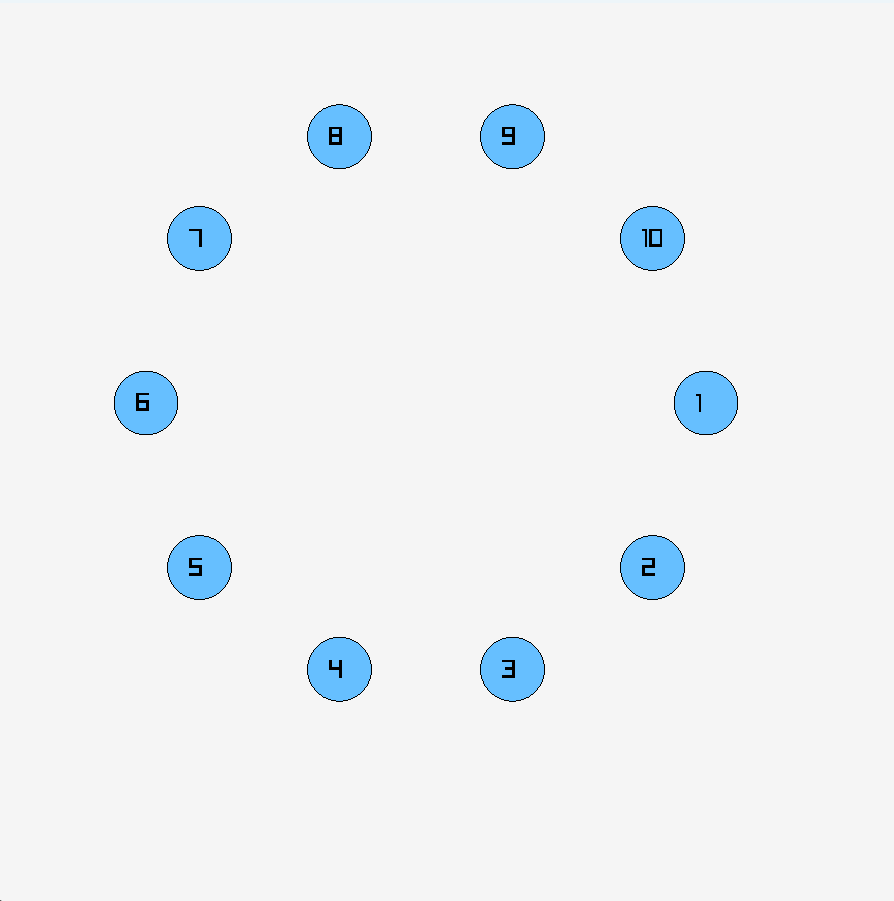
\includegraphics[width=0.9\textwidth]{Picture/hinh2_do_thi_quy_dao.png}
    \fbox{\begin{minipage}{0.8\textwidth}\centering\vspace{2cm}\textbf{[CHƯA TẢI ẢNH GIAO DIỆN ĐỒ THỊ - BỎ COMMENT ĐỂ HIỂN THỊ]}\vspace{2cm}\end{minipage}}
    \caption{Giao diện đồ họa phân bố hệ thống các đỉnh theo quỹ đạo đồng tâm}
    \label{fig:do_thi_quy_dao}
\end{figure}

\subsection{Kết quả thực thi của chương trình}
Trong suốt quá trình phần mềm thực thi, nhãn thông tin khoảng cách $L$ cập nhật liên tục dưới chân từng nút tròn. Sắc xanh lá đại diện cho đỉnh đã tối ưu hoàn toàn, sắc vàng biểu thị đỉnh đang đóng vai trò tâm loang xét duyệt hiện tại. Bất kỳ sự thay đổi nào cũng được ghi nhận vào bảng Log bên phải.

\begin{figure}[H]
    \centering
    % 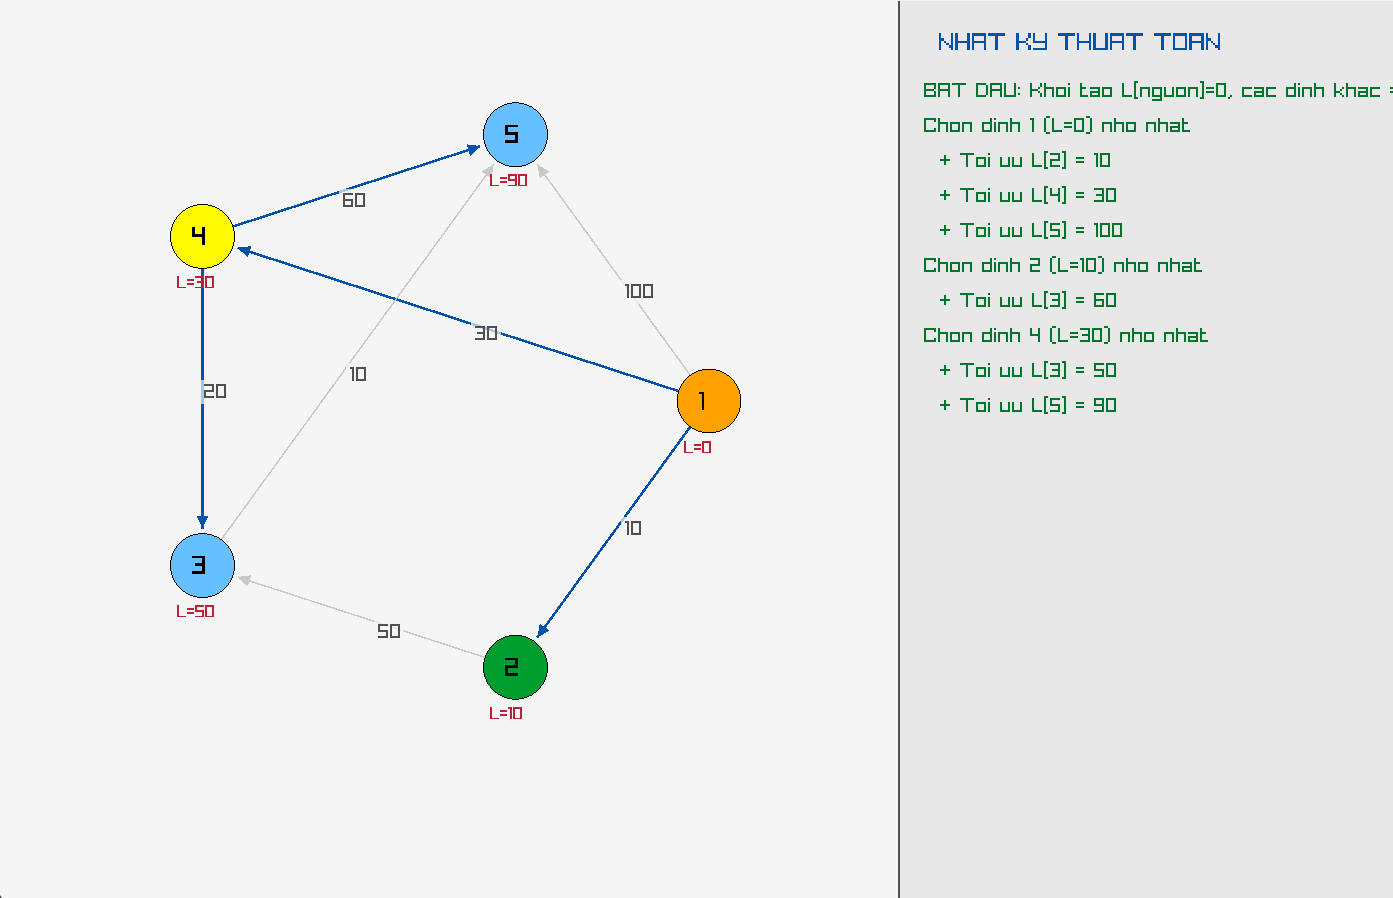
\includegraphics[width=0.9\textwidth]{Picture/hinh3_nhat_ky_thuat_toan.png}
    \fbox{\begin{minipage}{0.8\textwidth}\centering\vspace{2cm}\textbf{[CHƯA TẢI ẢNH NHẬT KÝ - BỎ COMMENT ĐỂ HIỂN THỊ]}\vspace{2cm}\end{minipage}}
    \caption{Bảng điều khiển nhật ký hoạt động cập nhật trạng thái loang nhãn từng bước}
    \label{fig:nhat_ky_thuat_toan}
\end{figure}

Khi tìm thấy đích, toàn bộ các cạnh và đỉnh cấu thành đường đi ngắn nhất tự động chuyển đổi sắc màu hiển thị sang màu đỏ rực rỡ với độ dày nét vẽ vượt trội nhằm cô lập lộ trình trực quan cho người sử dụng.

\begin{figure}[H]
    \centering
    % 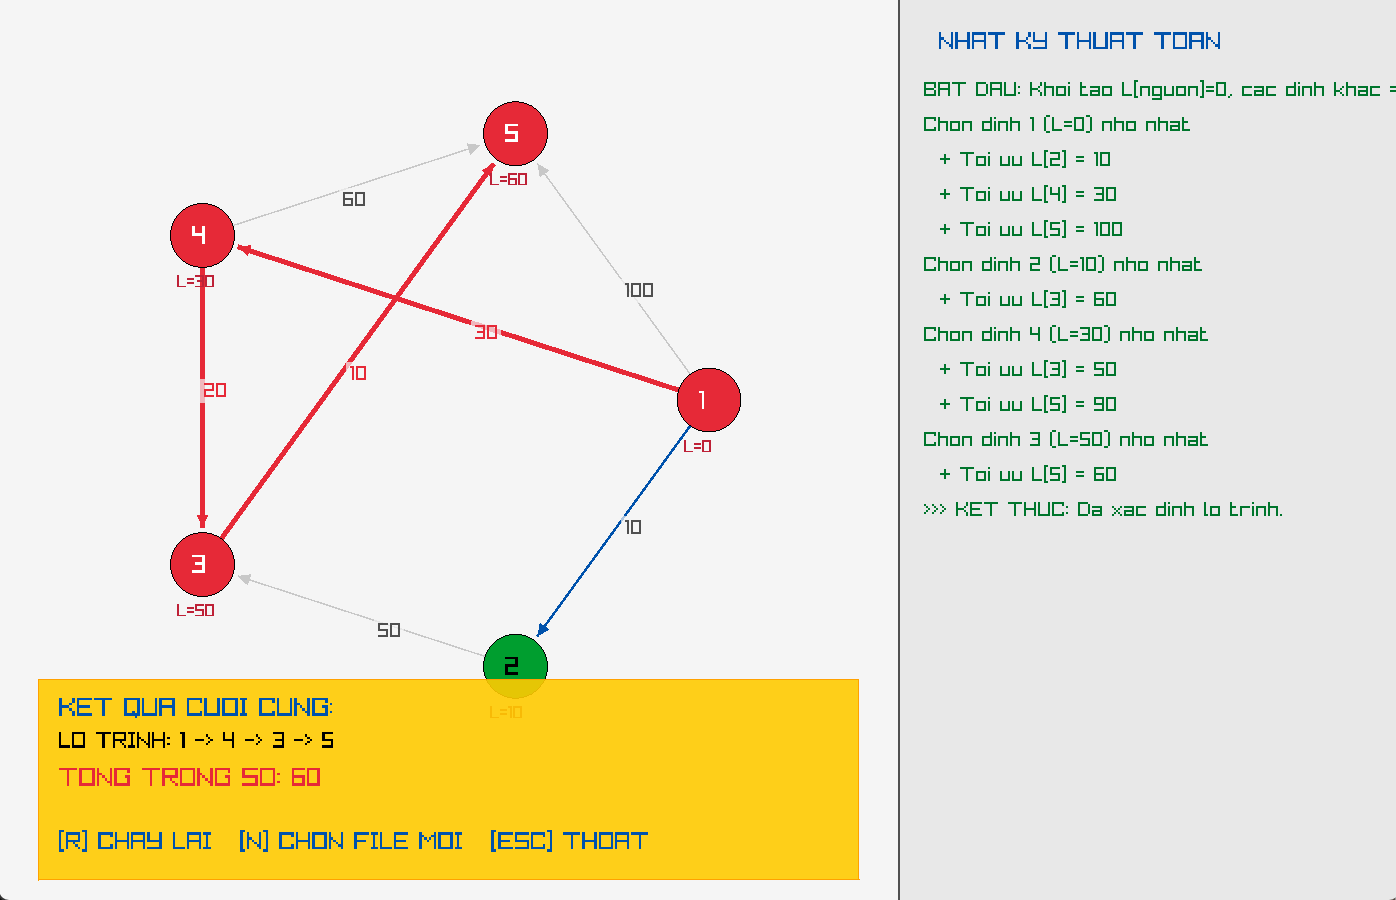
\includegraphics[width=0.9\textwidth]{Picture/hinh4_ket_qua_lo_trinh.png}
    \fbox{\begin{minipage}{0.8\textwidth}\centering\vspace{2cm}\textbf{[CHƯA TẢI ẢNH KẾT QUẢ - BỎ COMMENT ĐỂ HIỂN THỊ]}\vspace{2cm}\end{minipage}}
    \caption{Biểu diễn lộ trình ngắn nhất bằng hiệu ứng đổi màu cung liên kết sang sắc đỏ}
    \label{fig:ket_qua_lo_trinh}
\end{figure}

\subsection{Nhận xét đánh giá}
\textbf{Ưu điểm:} Ứng dụng giải quyết triệt để bài toán tìm kiếm tối ưu trên mô hình đồ thị có hướng phức tạp. Thiết kế giao diện đồ họa có tính tương tác cao, cơ chế máy trạng thái phân rã logic vận hành trơn tru và trực quan hóa sâu sắc dữ liệu từng bước chạy. Không xảy ra rò rỉ bộ nhớ (Memory Leak) nhờ sử dụng hạ tầng mảng cấp phát tĩnh.

\textbf{Hạn chế tồn tại:} 
\begin{itemize}
    \item Chương trình hiện tại yêu cầu dữ liệu tệp tin văn bản đầu vào phải tuân thủ nghiêm ngặt cấu trúc định dạng chuẩn hóa sẵn, chưa có cơ chế kiểm lỗi ngoại lệ mạnh mẽ.
    \item Thao tác tìm kiếm đỉnh Min hiện tại đang dùng cấu trúc duyệt tuyến tính $O(V)$ cho mỗi bước. Do đó tổng độ phức tạp thuật toán đang ở ngưỡng $O(V^2)$. Đây là điểm yếu nếu đồ thị có hàng chục ngàn đỉnh.
\end{itemize}

% ==================== CHƯƠNG 5 ====================
\chapter{KẾT LUẬN VÀ HƯỚNG PHÁT TRIỂN}

\section{Kết luận}
Qua quá trình nỗ lực nghiên cứu và hoàn thiện đồ án PBL1, nhóm sinh viên đã củng cố thành công nền tảng cấu trúc dữ liệu tĩnh và làm chủ giải thuật cốt lõi Dijkstra. Việc áp dụng thành công kỹ thuật hình học lượng giác và thư viện Raylib vào kiến trúc Máy trạng thái phân mảnh đã giúp chương trình vận hành chính xác, minh họa trực quan sinh động tiến trình loang nhãn phức tạp của hệ thống đồ thị.

\section{Hướng phát triển}
\begin{itemize}
    \item Khắc phục độ phức tạp $O(V^2)$ bằng cách nâng cấp cấu trúc mảng duyệt tuần tự thành Hàng đợi ưu tiên (Min-Heap), giúp giảm độ phức tạp thời gian về ngưỡng $O(E \log V)$.
    \item Phát triển Module kéo thả tương tác chuột trên màn hình, cho phép người dùng tự do vẽ đỉnh, nối cung đồ thị bằng thao tác Click thay vì phải nhập liệu tệp văn bản.
    \item Tối ưu hoá hình vẽ đồ thị cho dữ liệu lớn, minh hoạ rõ ràng, trực quan hơn.
    \item Tích hợp song song giải thuật Bellman-Ford để so sánh trực quan thời gian chạy và khả năng xử lý đồ thị chứa trọng số âm.
\end{itemize}

% ==================== TÀI LIỆU THAM KHẢO ====================
\newpage
\addcontentsline{toc}{chapter}{TÀI LIỆU THAM KHẢO}
\begin{thebibliography}{9}
\bibitem{ref1} 
Nguyễn Đức Nghĩa, \textit{Giáo trình Toán rời rạc}, Nhà xuất bản Bách Khoa Hà Nội.
\bibitem{ref2} 
Phan Thanh Tao, \textit{Giáo trình Toán rời rạc}, Trường Đại học Bách Khoa – Đại học Đà Nẵng.
\bibitem{ref3} 
Thomas H. Cormen, Charles E. Leiserson, Ronald L. Rivest, and Clifford Stein, \textit{Introduction to Algorithms}, MIT Press.
\bibitem{ref4} 
Raylib Graph Graphics Development Documentation, \url{https://www.raylib.com/}.
\bibitem{ref5}
Nguyễn Văn Hiệu, \textit{Bài toán đường đi ngắn nhất trên đồ thị}, Trường Đại học Bách Khoa - Đại học Đà Nẵng.
\bibitem{ref6}
Nguyễn Văn Hiệu, \textit{Tập bài giảng Toán rời rạc}, Trường Đại học Bách Khoa - Đại học Đà Nẵng.
\end{thebibliography}

% ==================== PHỤ LỤC MÃ NGUỒN CỐT LÕI ====================
\newpage
\chapter*{PHỤ LỤC}
\addcontentsline{toc}{chapter}{PHỤ LỤC}

% --- HIGHLIGHT BOX CHO GITHUB REPO ---
\begin{tcolorbox}[
    colback=blue!5!white,
    colframe=blue!75!black,
    title=\textbf{MÃ NGUỒN DỰ ÁN (GITHUB)},
    fonttitle=\bfseries,
    rounded corners,
    arc=4pt,
    boxrule=1pt,
    halign=center
]
    Toàn bộ mã nguồn, cách cài đặt, cách sử dụng đồ án được lưu trữ tại:\\
    \href{https://github.com/raii-cod/PBL-1}{\textbf{\color{blue}https://github.com/raii-cod/PBL-1}}
\end{tcolorbox}
\vspace{1cm}

\section*{Trích đoạn các hàm xử lý cốt lõi của ứng dụng}

\subsection*{1. Động cơ phân mảnh Máy trạng thái Dijkstra:}
\begin{lstlisting}[style=UserCStyle]
if (state == STATE_FIND_MIN) {
    int min_d = INF; currentV = -1;
    for (int i = 1; i <= g.n; i++)
        if (g.T[i] && g.L[i] < min_d) { min_d = g.L[i]; currentV = i; }

    if (currentV == -1 || currentV == v_target) {
        state = STATE_FINISHED;
        if (g.L[v_target] != INF) {
            int t = v_target;
            int temp[N], count = 0;
            while (t != -1) { onPath[t] = true; temp[count++] = t; t = g.par[t]; }
        }
        AddLog(">>> KET THUC: Da xac dinh lo trinh.", stepLogs, &logCount);
    } else {
        g.T[currentV] = 0; neighborIdx = 1; state = STATE_RELAX_EDGES;
    }
} 
else if (state == STATE_RELAX_EDGES) {
    bool found = false;
    while (neighborIdx <= g.n) {
        if (g.A[currentV][neighborIdx] != -1 && g.T[neighborIdx]) {
            int newD = g.L[currentV] + g.A[currentV][neighborIdx];
            if (newD < g.L[neighborIdx]) {
                g.L[neighborIdx] = newD;
                g.par[neighborIdx] = currentV;
            }
            neighborIdx++; found = true; break;
        }
        neighborIdx++;
    }
    if (!found) state = STATE_FIND_MIN;
}
\end{lstlisting}

\subsection*{2. Hàm tính toán vector dựng mũi tên:}
\begin{lstlisting}[style=UserCStyle]
void drawArrow(Vector2 start, Vector2 end, float rDinh, Color mau, int trongSo) {
    float angle = atan2f(end.y - start.y, end.x - start.x);
    Vector2 tip = { end.x - (rDinh + 5) * cosf(angle), end.y - (rDinh + 5) * sinf(angle) };
    DrawLineEx(start, tip, 2.0f, mau);
    
    float arrowSize = 14.0f;
    Vector2 p1 = { tip.x + arrowSize * cosf(angle + PI - 0.45f), tip.y + arrowSize * sinf(angle + PI - 0.45f) };
    Vector2 p2 = { tip.x + arrowSize * cosf(angle + PI + 0.45f), tip.y + arrowSize * sinf(angle + PI + 0.45f) };
    DrawTriangle(tip, p2, p1, mau); 
}
\end{lstlisting}

\end{document}